\section{Durchführung}
\label{sec:Durchführung}

% Was wurde gemessen bzw. welche Größen wurden variiert?

\subsection{Bestimmung der Untergrundrate}
\label{ssec:d1}

Das erste Problem der Messung ist die Umgebungsradioaktivität, diese sollte so niedrig wie möglich gehalten werden.
Dennoch muss diese Grundstrahlung aus den späteren Berechnungen herausgerechnet werden können. 
Dafür wird zunächst die Untergrundrate $N_\text{U}$ berechnet. 
Für alle weiteren Versuche wird der Versuchsaufbau aus \autoref{fig:aufbau} verwendet.

\begin{figure}
    \centering
    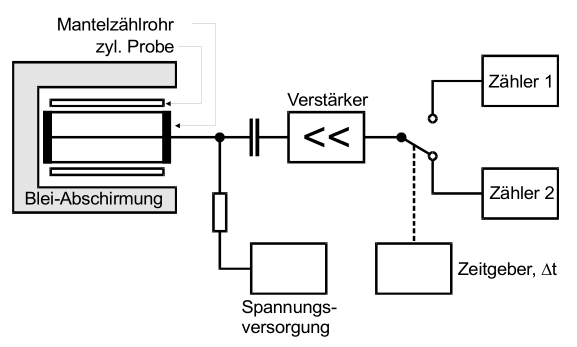
\includegraphics[width=0.6\textwidth]{images/bild3.png}
    \caption{Schematischer Aufbau des Versuchs.}
    \label{fig:aufbau}
\end{figure}

In der Nullmessung, wird keine Probe eingesetzt.
Für $\SI{300}{\second}$ wird $N_\text{U}$ sieben mal gemessen und die Zählrate notiert.

\subsection{Bestimmung der Halbwertszeit von Vanadium}
\label{ssec:d2}

Es wird eine zerfallende Vanadium-Probe mit einer Apperatur wie in \autoref{fig:therm} erzeugt und dann sofort in die Messapperatur gesteckt. 
Mit einer Integrationszeit von $\SI{30}{\second}$ werden dann die Zerfälle gemessen.
Nach $\SI{1230}{\second}$ wird die Messung beendet.

\subsection{Bestimmung der Halbwertszeit von Rhodium}
\label{ssec:d3}

Für Rhodium wird die gleiche Messung wie für Vanadium durchgeführt.
Der Unterschied ist hierbei, dass die Integrationszeit $\SI{15}{\second}$ beträgt und dementsprechend bis $\SI{630}{\second}$ gemessen wird.